% !TEX root =../thesis.tex
\chapter{Tycho's Six: High-Resolution spectroscopy search for the remaining donor for the Tycho supernova}
\label{chap:sn1572_hires}

% TITLE AND AUTHORS
%-----------
%\title{Tycho's Six: High-Resolution spectroscopy search for the remaining donor for the Tycho supernova\footnotemark{1}}

\section{Introduction}
\label{sec:introduction}


Type Ia Supernovae (\sneia) are of great interest for astronomy. They have a plethora of applications in stellar and galactic astronomy as well as in cosmology. Despite their significance, little is known about the progenitor of these events. 

There is general consensus that \sneia\ are caused by the deflagration/detonation of a CO white dwarf approaching the Chandrasekhar mass (1.38 M$_{\odot}$). The necessary accretion process, increasing the white dwarf's mass to the Chandrasekhar mass, however remains a mystery.

The community has proposed two main scenarios for this accretion process. The first scenario sees the accretion process happening through Roche Lobe Overflow (henceforth RLOF) of a close companion (also known as donor star). This companion, which underwent common envelope evolution with the white dwarf, is a main-sequence to red giant star at the time of the explosion (\sd\ scenario). The donor star survives the explosion and remains visible post-explosion.

The second scenario is the merger of two white dwarfs (\dd\ scenario). In most cases this would leave no remaining star \citep[e.g.][]{2010Natur.463...61P}.

Both scenarios have support in observation and theory. The detection of circum-stellar material around SN2006X \citep{2007Sci...317..924P} provides support for the \sd\ model. On the other hand the lack of substantial hydrogen in most other \sneia\ \citep{2007ApJ...670.1275L} poses a challenge to the \sd\ scenario.


\citet{2010ApJ...708.1025K} suggests a UV-excess for the \sd\ scenario in early times of the light curve. This excess is caused by the collision of the supernova ejecta with the companion. Such an excess has not yet been observed \citep{2010ApJ...722.1691H}. 

Furthermore recent population synthesis calculations \citep{2009ApJ...699.2026R, 2010A&A...515A..89M,2010A&A...521A..85Y} suggest 
that the \sd\ scenario can not explain the observed \sneia\ rates. However the \dd\ scenario also does not produce enough \sneia. The authors suggest a population comprising of single and double degenerate \sneia. 


For most scenarios a white dwarf merger will lead to the formation of a neutron star \citep{1985A&A...150L..21S}. However \citet{2010Natur.463...61P} have shown that for certain parameters (white dwarf binaries with a mass ratio very close to one) the merger may explain sub-luminous supernovae. 

To solve the progenitor question, at least for a few \sneia, \citet[][henceforth \rl]{2004Natur.431.1069R} have tried to directly detect donor stars in \snia\ remnants. Tycho's supernova remnant (SNR1572 henceforth) is well suited for this task. The remnant is relatively close ($2.8\pm0.8$\,kpc), very young and has been confirmed as a normal \snia\ remnant \citep{2006ApJ...645.1373B, 2008Natur.456..617K}. 

\rl\ found a star with an unusual spatial motion (\starg\ by their nomenclature) and suggested this as a possible donor star for SN1572. 

Our team used high resolution spectroscopy to confirm \rl's results for \starg\ \citep[][henceforth \wek]{2009ApJ...701.1665K}. We measured the spatial velocity but could not confirm the large unusual velocity determined by \rl. 

A previously overlooked consequence of RLOF is the rotational velocity induced by the tidal locking of the companion. This results in an unusually large rotationally velocity which might single out donor stars against nearby unrelated stars. We explored this for \starg\ in \wek\ but did not find an unusually large rotational velocity. \starg\ has all the characteristics of a background interloper, but we could not rule out a possible, yet contrived, involvement in SN1572.

\citet[henceforth \gh]{2009ApJ...691....1H} analysed a spectrum of \starg\ observed with the HIRES-instrument on the Keck telescope. \gh\ confirmed \wek's radial velocity . They determined stellar parameters and metallicities for \starg\ and concluded that \starg\ has an unusually large amount of Ni. \gh\ claim that this Ni measurement could be attributed to the accretion of ejecta material on the donor star. 

In this work we analyze the same HIRES spectrum of \starg\ as \gh. We also analyse Keck spectra (obtained with the same setup as \starg) of five other stars in SNR1572. 

The observation and data reduction is described in section \ref{sec:observ-data-reduct}. Section \ref{sec:analysis} is divided into five subsections detailing the measurements of proper motion, radial velocity, rotation, stellar parameters and abundances. We conclude this paper in section \ref{sec:conclusion}.



\section{Observations and Data Reduction}
\label{sec:observ-data-reduct}

We obtained spectra with the High Resolution Echelle Spectrograph \citep[HIRES][]{1994SPIE.2198..362V} on the Keck 10m telescope in Mauna Kea. The observations were done on two runs on 2006 09 10 and 2006 10 11.  The slits B5 and C1 (with the same width of 0.86\arcsec\ but different lengths, B5 length 3.5\arcsec, C1 length 7.0 \arcsec) were used resulting in a wavelength coverage of 3930 -- 5330 \AA, 5380 -- 6920 \AA\ and 6980 -- 8560 \AA\ with $R\approx 50,000$. This gave us the necessary spectral resolution and wavelength coverage to determine stellar parameters. 
The spectra were reduced using the MAKEE package. All spectra were heliocentrically corrected, using the MAKEE skyline method. The spectra were not corrected for telluric lines as they will not influence our analysis of the stellar parameters. The final exposure times of the combined spectra for each candidate and Signal to Noise ratio at 4000-4100 \AA\ are shown in Table \ref{tab:candexpo}. Finally we normalized the spectrum using the IRAF-Task continuum. We note that \starc\ and \stard\ were observed on the same slit (C1) with a separation of 2.1\,\arcsec.




%\begin{deluxetable}{ccccccc}
%
%\tablecaption{Observations of Stars}
%
%\tablehead{\colhead{Name} & \colhead{RA (J2000)} & \colhead{Dec (J2000)}  & \colhead{Date} & \colhead{Slit} & \colhead{$t_{\rm exp}$}& \colhead{S/N}\\
%\colhead{} & \colhead{(hh:mm:ss.ss)} & \colhead{(dd:mm:ss.ss)} & \colhead{(dd/mm/yy)} & \colhead{} & \colhead{(1)}}
%
%\startdata
%\stara & 00:25:19.73 & +64:08:19.6 & 10/09/06 & B5& 0.25 &$ \approx 65$ \\ \hline
%\starb & 00:25:19.95 & +64:08:17.11 & 10/09/06 & B5 & 0.25 &$ \approx 50$ \\ \hline
%\starc & 00:25:20.40 & +64:08:12.32 & 11/10/06 & C1 &0.25 & $ \approx 10$\\ \hline
%\stard & 00:25:20.60 & +64:08:10.82 & 11/10/06 & C1 &0.25 &10 \\ \hline
%\stare & 00:25:18.29 & +64:08:16.12 & 11/10/06 & C1 &0.25 & $\approx 15$\\ \hline
%\starg & 00:25:23.58 & +64:08:02.06 & 10/09/06 \& 11/10/06  & B5\&C1 &0.25& $\approx 30$\\ \hline
%\enddata
%
%\label{tab:candexpo}
%\end{deluxetable}

In addition, we obtained low-resolution spectroscopy ($R\approx1200$) of
\starb\ with the dual-arm Low-Resolution Imaging Spectrometer \citep[LRIS;][]{Oke95} mounted on the 10-m Keck I telescope. The
observations were taken on one run on 2010 11 07, using only the blue
arm with the 600/4000 grism and the 1\arcsec\ wide slit. This resulted
in a wavelength coverage of 3200--5600\,\AA. These observations
were taken to precisely measure the surface gravity for \starb.
The spectrum of \starb\ was reduced using standard techniques \citep[e.g.][]{Foley03}. Routine CCD processing and spectrum extraction
were completed with IRAF\footnote{IRAF: the Image Reduction and
Analysis Facility is distributed by the National Optical Astronomy
Observatory, which is operated by the Association of Universities for
Research in Astronomy (AURA) under cooperative agreement with the
National Science Foundation (NSF).}, and the data were extracted with
the optimal algorithm of \citet{Horne86}. We obtained the wavelength
scale from low-order polynomial fits to calibration-lamp spectra.
Small wavelength shifts were then applied to the data after measuring the offset by
cross-correlating a template sky to the night-sky lines that were
extracted with the star. Using our own IDL routines, we fit a
spectrophotometric standard-star spectrum to the data in order to flux
calibrate \starb\ and remove telluric lines \citep{Horne86,Matheson00}.


\section{Analysis}
\label{sec:analysis}

We tried to use the same analysis techniques for all star to receive a homogeneous dataset. For \starb\, however, we needed to switch to different techniques as it is much hotter than the rest of the candidates. In addition, \stard\ was not studied as extensively as the rest of the candidates due to the relatively poor quality of the spectrum (S/N ~ ??? 5)




\subsection{Astrometry}
\label{sec:propmot}
Peculiar proper motions can be used to identify potential donor stars. \rl\ suggested \starg\ as a possible donor due to its relatively high proper motion and radial velocity. For this work we measured proper motions for 124 stars within one arcminute of the remnant's center. We used archival HST images for 3 different epochs (HST Program ID  9729 \& 10098; November 2003, August 2004, May 2005) each consisting of 3 exposures of different lengths. This results in a maximum baseline of 30 months. Some faint stars where not detected in the shorter exposures and were thus excluded from proper motion measurements.


We used an image from the middle epoch (2004) to establish a reference frame and oriented the pixel coordinate system with the equatorial system. The scale of this reference image is 50\,mas\,pixel$^{-1}$. We then applied a distortion correction for the F555W filter \citep{2006acs..rept....1A} to the images and calculated transformations between all other images and the reference image. We used these transformations to calculate the position of all stars in the reference coordinate system.


Finally, we used a standard Levenberg-Marquardt solver \citescipy\ to do a linear regression for stellar positions in the pixel coordinates x and y (which are lined up with the equatorial coordinates). In this case we treated the measurement in x and y as independent measurements. The errors were obtained by $\chi^2$ analysis. Table \ref{tab:propmot} lists the proper motions and errors of all stars mentioned in \rl\ which were analyzed in this work. In Figure \ref{fig:propmot} we have compared the proper motion of all stars analyzed for proper motion and the program stars close to the remnant's center.

\begin{figure}[htbp] %  figure placement: here, top, bottom, or page
   \centering
   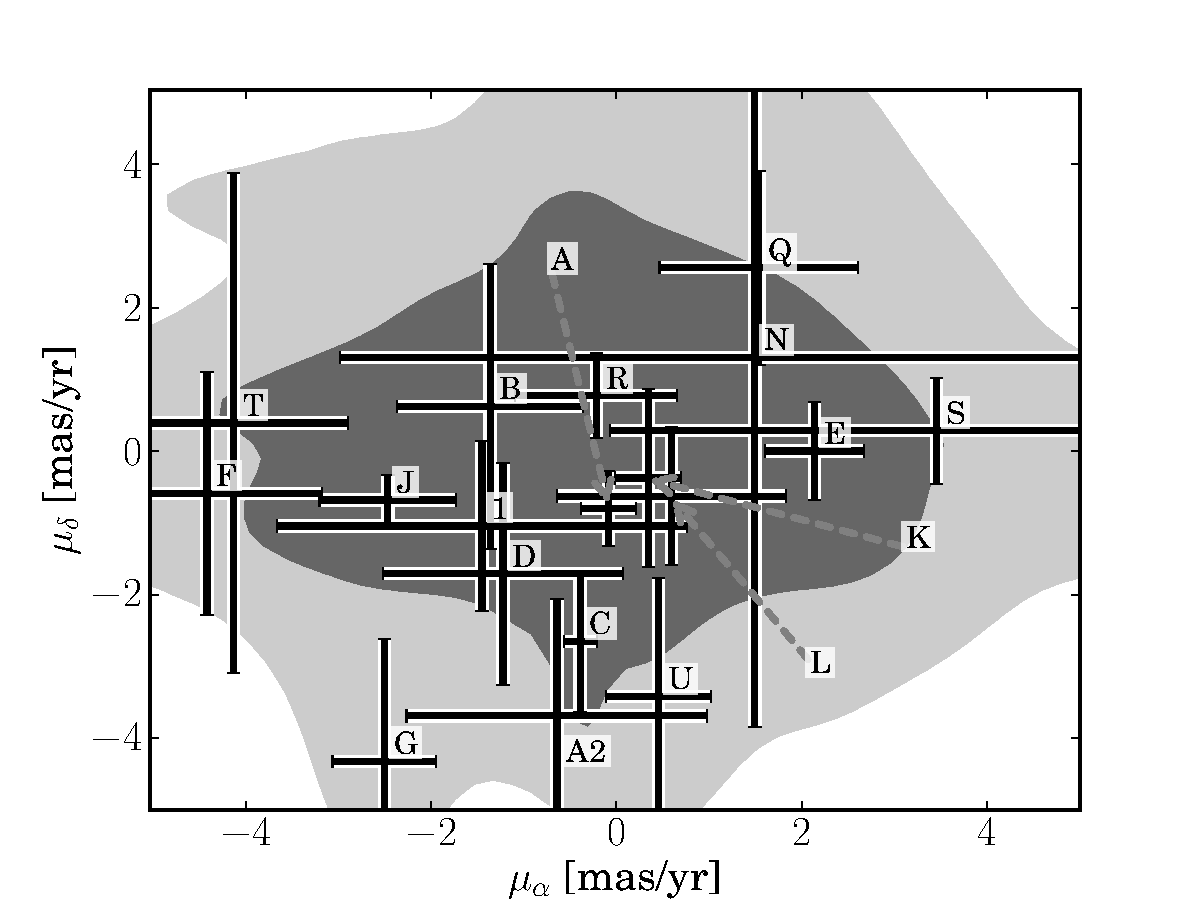
\includegraphics[width=0.5\textwidth]{chapter3/plots/propmot_distr.pdf} 
   \caption{The gray scale shows the underlying proper motion distribution of all stars. The data of a select set of stars is shown including errors on top of the contours. We note that \starg\ and \staraii\ are outliers. Tycho-2 was not shown in this figure as it is an extreme outlier with $\mu_\alpha=75$\,\masyr\ and $\mu_\delta=-4.4$\,\masyr\ but also at a large distance to the center of the remnant.}
   \label{fig:propmot}
\end{figure}

%\begin{deluxetable}{ccccccc}

%\tablecaption{Proper motion of Candidates}
%
%\tablehead{\colhead{Name} & \colhead{RA (J2000)} & \colhead{Dec (J2000)}  & \colhead{$\mu_\alpha$} & \colhead{$\mu_\delta$} & \colhead{$\Delta\,\mu_\alpha$}& \colhead{$\Delta\,\mu_\delta$}\\
%\colhead{} & \colhead{(hh:mm:ss.ss)} & \colhead{(dd:mm:ss.s)} & \colhead{mas\,yr$^{-1}$} & \colhead{mas\,yr$^{-1}$} & \colhead{mas\,yr$^{-1}$} & \colhead{mas\,yr$^{-1}$}}
%
%\startdata
%Tycho-1&0:25:16.69&+64:08:12.4&-1.45&-1.04&2.21&1.18\\
%Tycho-2&0:25:22.45&+64:07:32.5&75.05&-4.39&0.51&1.65\\
%Tycho-9&0:25:24.31&+64:08:40.5&0.60&-0.63&1.24&0.96\\
%\stara&0:25:19.73&+64:08:19.6&-0.08&-0.80&0.30&0.52\\
%Tycho-A2&0:25:19.80&+64:08:19.9&-0.64&-3.69&1.62&1.63\\
%\starb&0:25:19.95&+64:08:17.1&-1.36&0.62&1.00&1.99\\
%\starc&0:25:20.40&+64:08:12.3&-0.39&-2.66&0.18&0.98\\
%\stard&0:25:20.60&+64:08:10.8&-1.22&-1.71&1.30&1.55\\
%\stare&0:25:18.29&+64:08:16.1&2.14&0.00&0.54&0.68\\
%Tycho-F&0:25:17.10&+64:08:31.0&-4.42&-0.59&1.24&1.70\\
%\starg&0:25:23.58&+64:08:02.0&-2.50&-4.33&0.56&1.70\\
%Tycho-J&0:25:15.08&+64:08:06.0&-2.46&-0.68&0.74&0.35\\
%Tycho-K&0:25:23.89&+64:08:39.3&0.35&-0.38&0.36&1.24\\
%Tycho-L&0:25:24.31&+64:08:40.5&0.60&-0.63&1.24&0.96\\
%Tycho-N&0:25:14.74&+64:08:28.2&1.49&1.31&4.47&5.15\\
%Tycho-Q&0:25:14.81&+64:08:34.2&1.54&2.56&1.07&1.36\\
%Tycho-R&0:25:15.52&+64:08:35.4&-0.22&0.77&0.88&0.59\\
%Tycho-S&0:25:13.79&+64:08:34.5&3.45&0.29&3.53&0.74\\
%Tycho-T&0:25:14.59&+64:07:55.1&-4.13&0.39&1.23&3.48\\
%Tycho-U&0:25:19.25&+64:07:38.0&0.45&-3.42&0.57&1.66\\
%\enddata
%\label{tab:propmot}
%
%\end{deluxetable}

\subsection{Radial Velocity}
\label{sec:radvel}

The radial velocity of each star was measured using the IRAF task \textit{fxcor} \citep{1979AJ.....84.1511T}. MAKEE was used to calculate an intrinsic velocity shift by comparing offsets of the nightsky-lines. The radial velocity standards were reduced in the same fashion. 
 
Each order of each star was then cross-correlated with at least two other radial velocity standards (HR6349, HR6970, HR1283) which had been observed on the same night.


\paragraph{\starb:}
The radial velocity for \starb\ was measured in the course of determining the stellar parameters for \starb with \textit{sfit} \citesfit. The \textit{sfit} result consistently gives $v_{\textnormal{helio}} = -55$ \kms\ for different stellar parameters with an error of $\approx 2$\,\kms. 


In Table \ref{tab:radvel} we have listed all the radial velocities both in a heliocentric frame and a local-standard-of-rest (henceforth LSR) frame. We will be referring to the heliocentric measurements from here on. The listed error is the standard deviation of the radial velocity measurement of all orders added in quadrature to the error of the radial velocity standards.

In Figure \ref{fig:dist_vr} we have compared the radial velocity of our sample stars to radial velocities of stars in the direction of Tycho's SNR using the Besan\c{c}on Model \citep{2003A&A...409..523R}. The distance as well as the error in distance are taken from Section \ref{sec:distance}.  The candidates radial velocities are all typical for their distance. Finally, the measurement of \starg\ is consistent with \wek\ and \gh.

%\begin{deluxetable}{ccccc}
%\tablecaption{Radial velocities \label{tab:radvel}}
%\tablehead{\colhead{Name} & \colhead{Date} & \colhead{$v_{\textnormal{helio}}$} & \colhead{$v_{\textnormal{LSR}}$} &\colhead{$\Delta v$} \\
%\colhead{(-)} & \colhead{(dd/mm/yy)} & \colhead{(\kms)} & \colhead{(\kms)} & \colhead{(\kms)}}
%
%\startdata
%\stara & 09/09/06 & -36.79 & -28.5 & 0.23   \\
%\starb & 09/09/06 & -55.0 & -57.0 & $\approx 2$ \\
%\starc & 11/10/06 & -58.78 & -50.49 & 0.75   \\
%\stard & 11/10/06 & -58.93 & -50.64 & 0.78   \\
%\stare & 11/10/06 & -64.2 & -55.91 & 0.27   \\
%\starg & 09/09/06 & -87.12 & -78.83 & 0.25 \\
%\starg & 11/10/06 & -87.51 & -79.22 & 0.78 \\
%\enddata



%\end{deluxetable}

\begin{figure}[htbp] %  figure placement: here, top, bottom, or page
   \centering
   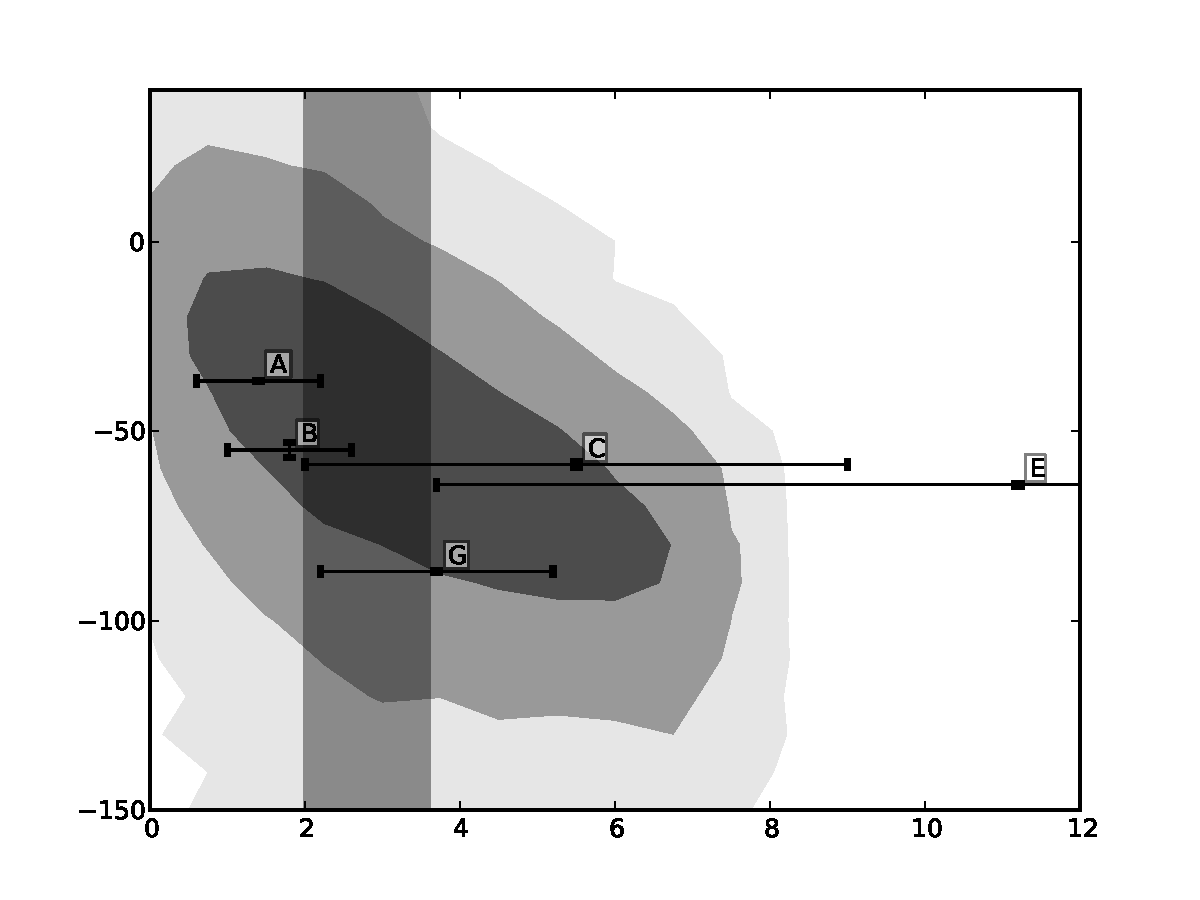
\includegraphics[width=0.5\textwidth]{chapter3/plots/dist_vr.pdf} 
   \caption{The contours indicate 1, 2 and $3-\sigma$ levels of the distance and radial velocity using the Besan\c{c}on Model \citep{2003A&A...409..523R} with 62,774 stars in the direction of SNR1572. We have overplotted our candidate stars with error bars. One should note that the errors in distance are only an indication of the error, the proper error surfaces can be seen in Figure \ref{fig:mc_isochrone}. The vertical gray shade shows the error range for the distance of SNR1572.}
   \label{fig:dist_vr}
\end{figure}



\subsection{Rotational Velocity}
\label{sec:rotation}
We have measured rotational velocities of all cool stars (\stara, \starc, \stare\ and \starg) in the same fashion as described in \wek. We selected several unblended and strong (but not saturated) \ion{Fe}{1} lines in the stellar spectra .  We added these lines after shifting them to the same wavelength and scaling them to the same equivalent width. This was done to improve the signal to noise ratio for the faint stars as well as providing consistency throughout all stars. 

 As a reference we created three synthetic spectra for each star (one broadened only with the instrumental profile, the others with the instrumental profile and $v_{\rm{rot}}\sin{i}$\ of 10 and 13\,\kms\ respectively) with the 2010 version of MOOG \citemoog, using this work's temperature, gravity and metallicity.  As input data to MOOG we used the \citet{2004astro.ph..5087C} atmospheric models and a line list from \citet{1995KurCD..23.....K}. We then applied the same process of line selection and adding as for the lines in the observed spectra. 
 
Figure \ref{fig:rotvel} shows the comparison between the synthetic spectra of different rotational velocity and the observed spectra. This comparison indicates that the stellar broadening (rotational, macro turbulence, etc. ) is less than broadening due to the instrumental profile of 6\,\kms\ for each star. We adopt 6\,\kms\ as an upper limit to the rotation for all stars.
In the case of \starg, if one were to adopt this works measurements of the
peculiar spatial motion (see sections \ref{sec:propmot} and \ref{sec:radvel}, it could be concluded that $\sin{i}$ is much closer
to 1 than 0 and thus that the rotational velocity is less than 6\,\kms.



\begin{figure*}[h!]
\begin{tabular}{cc}
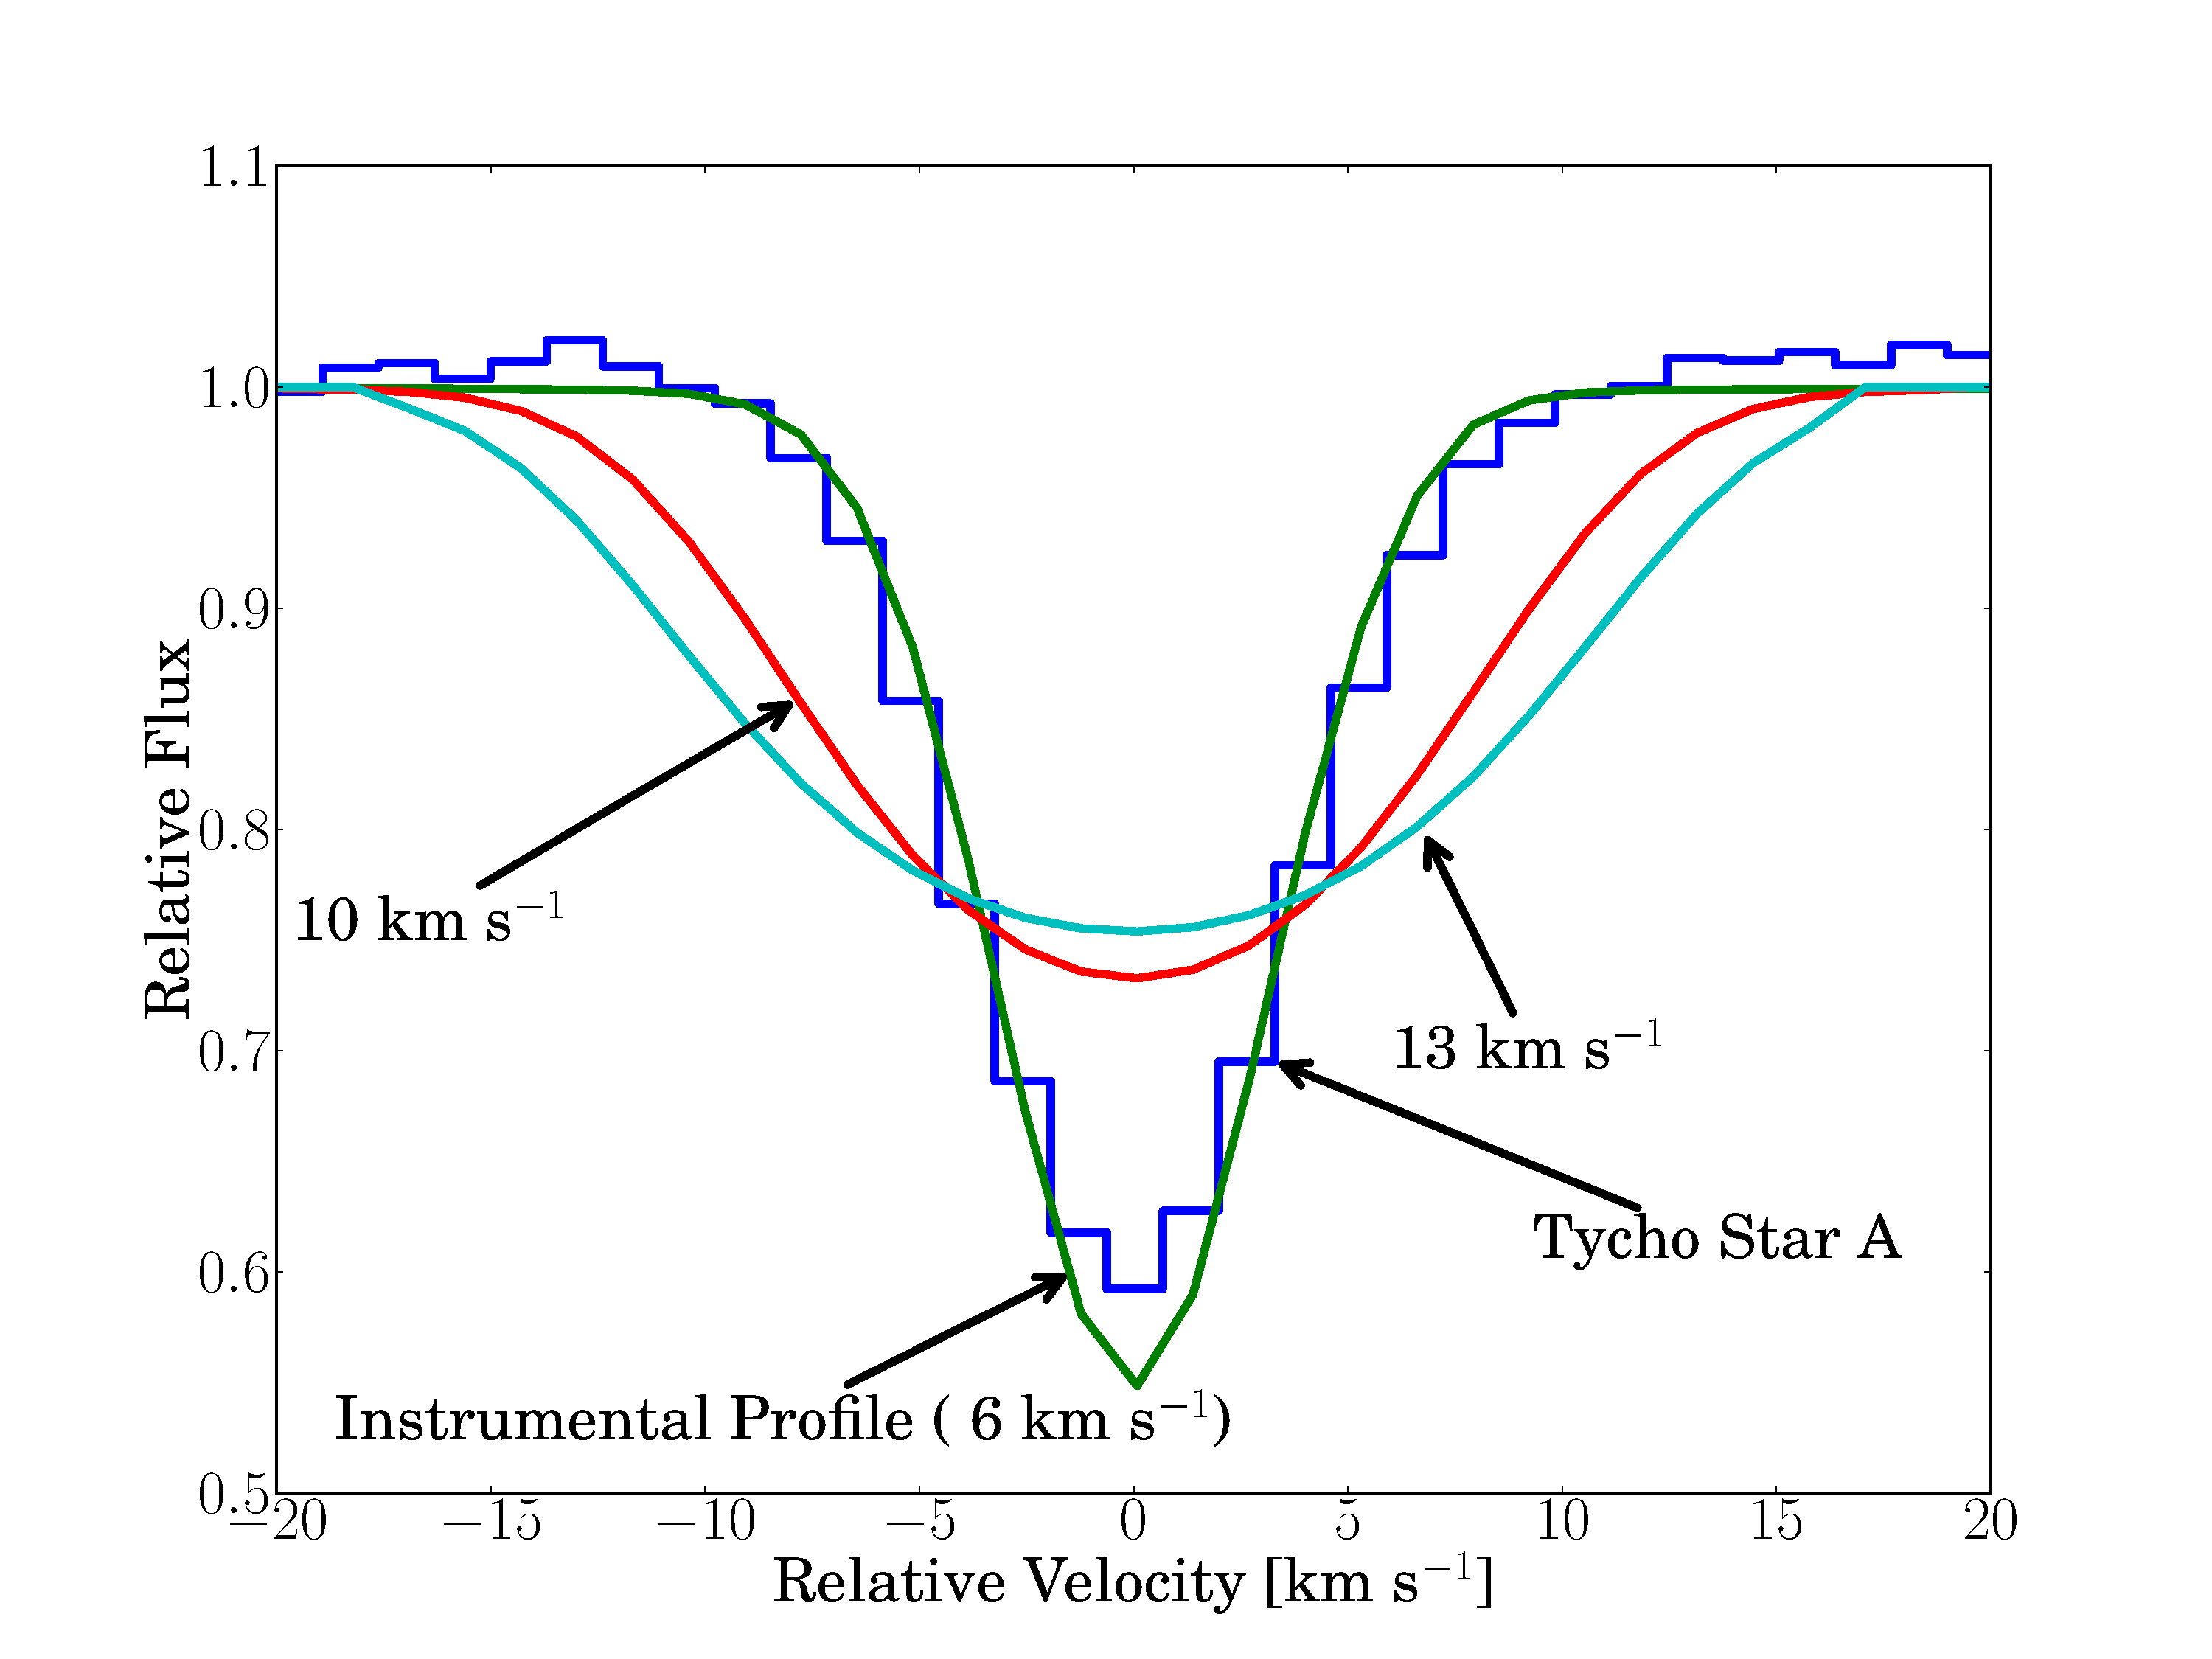
\includegraphics[width=0.45\textwidth, trim=130 30 60 0]{chapter3/plots/stara_rotation.pdf} &
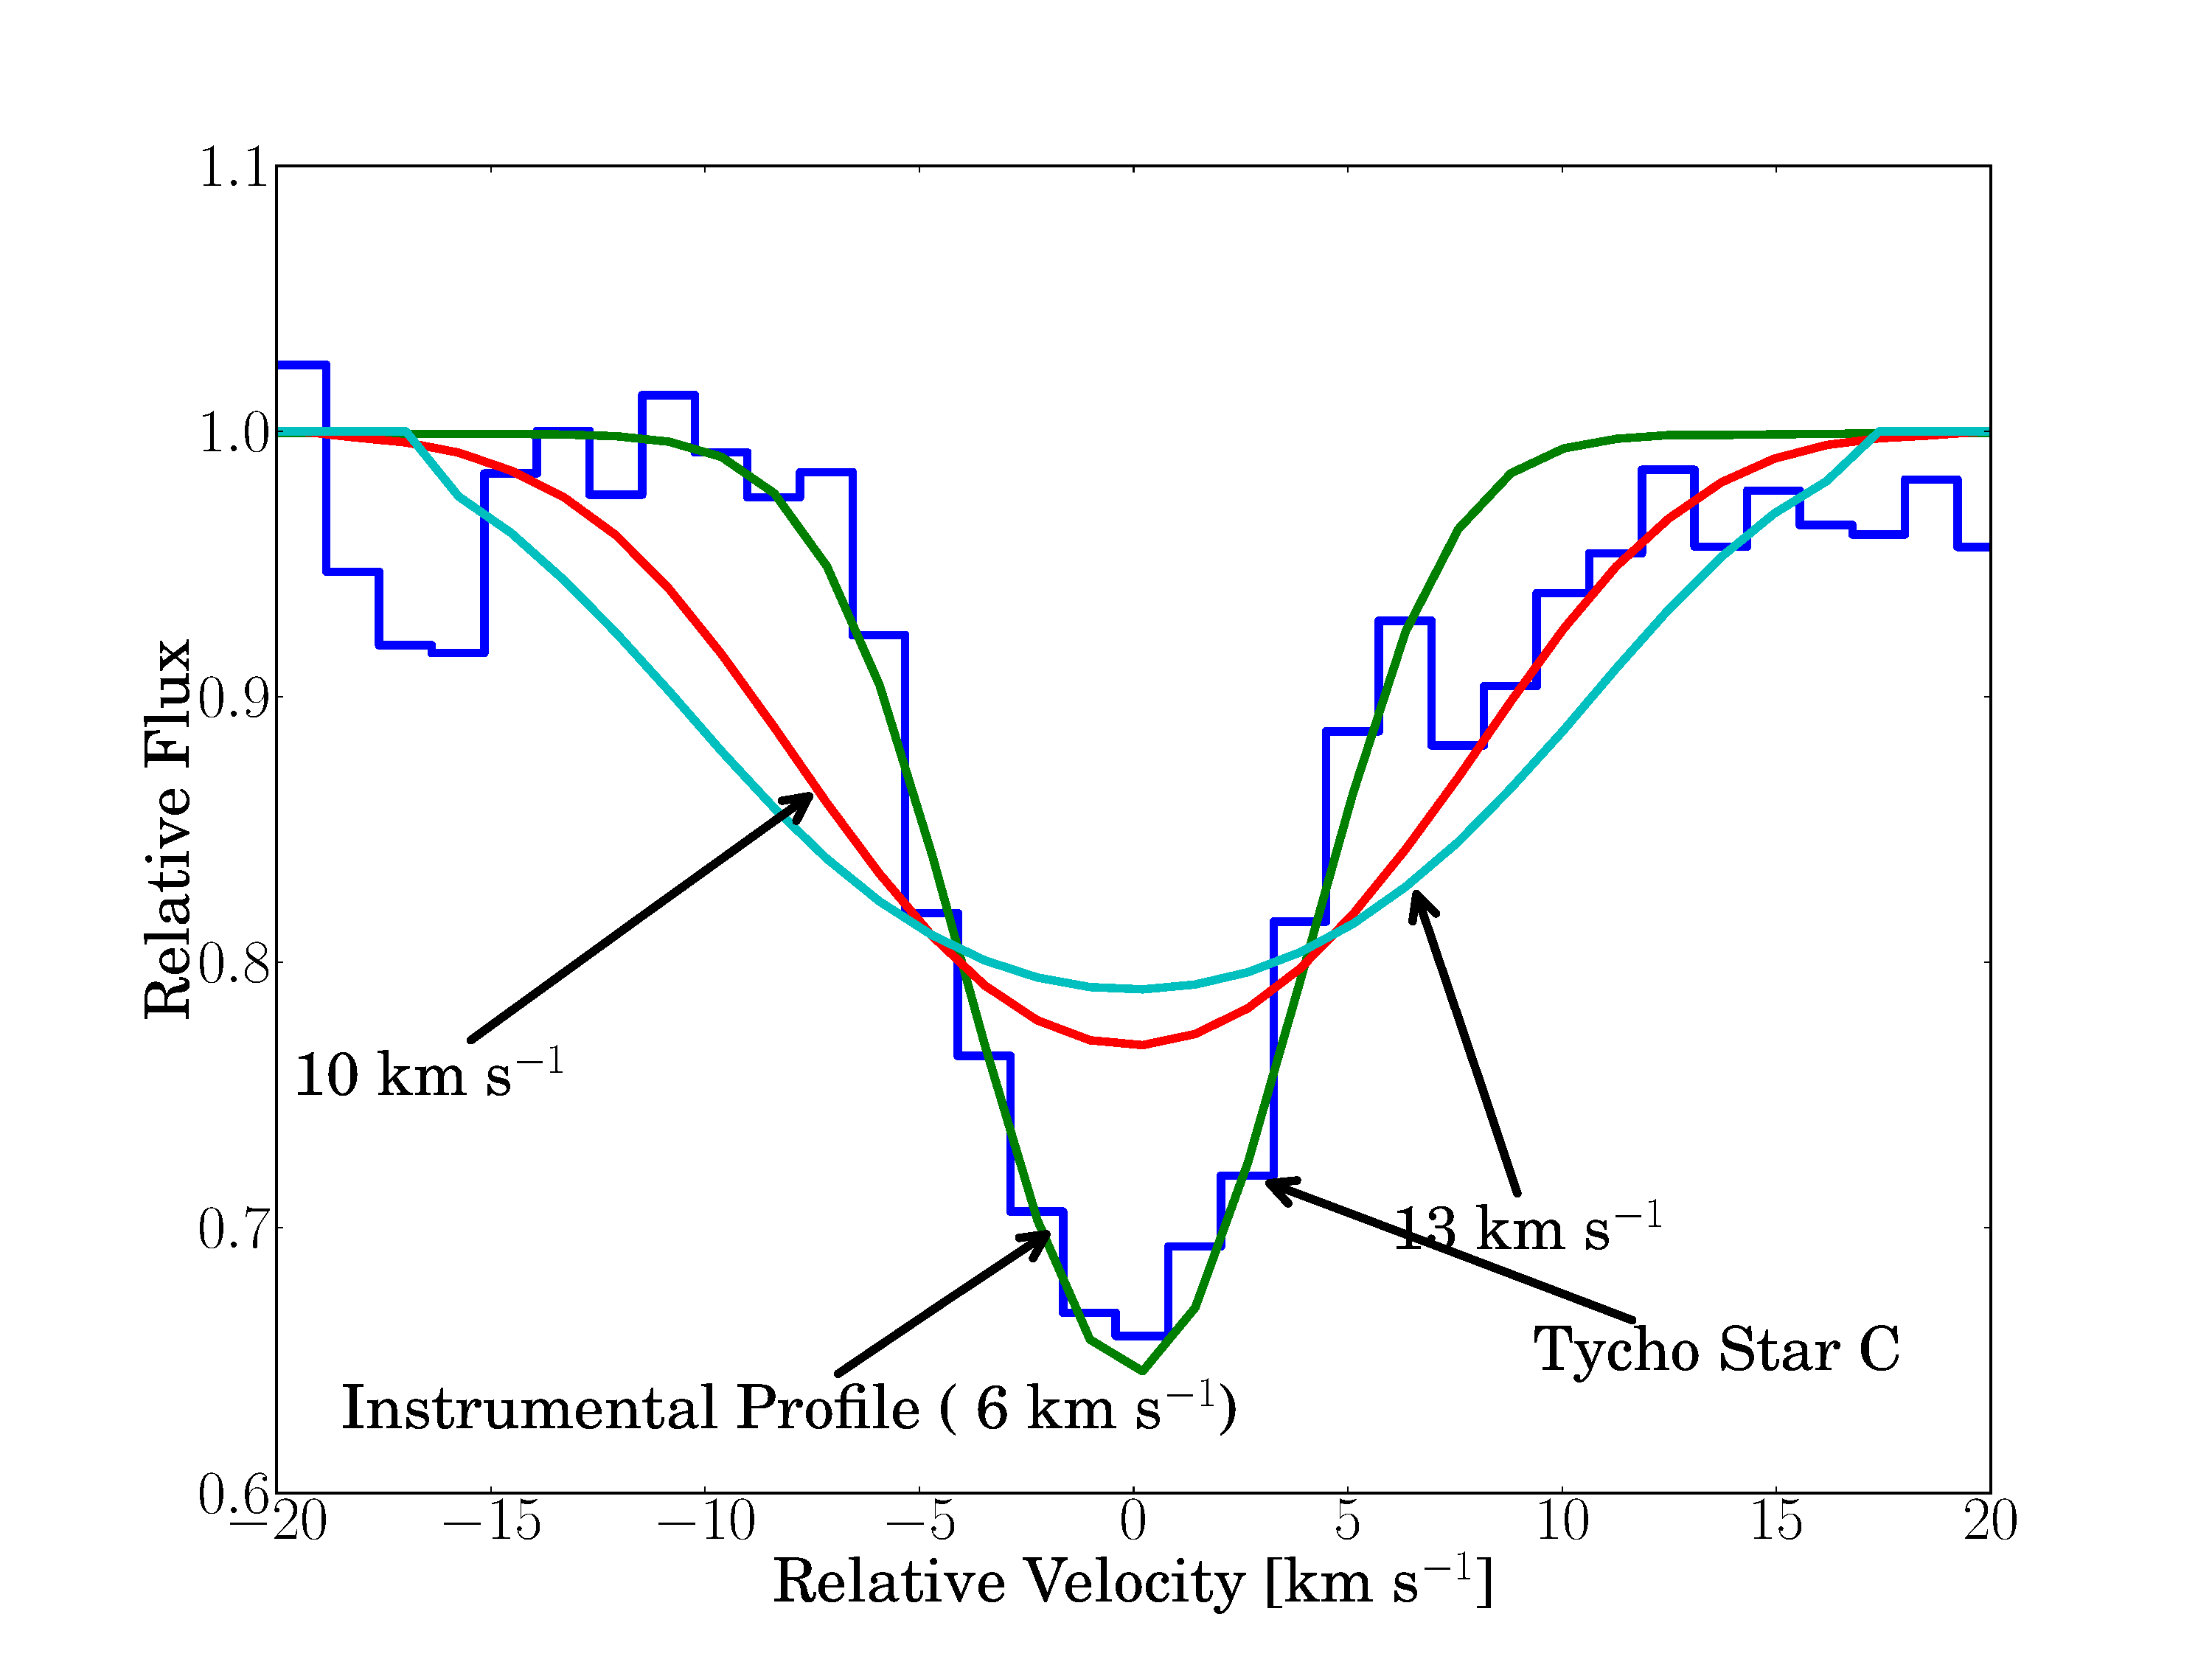
\includegraphics[width=0.45\textwidth, trim=130 30 60 0]{chapter3/plots/starc_rotation.pdf} \\
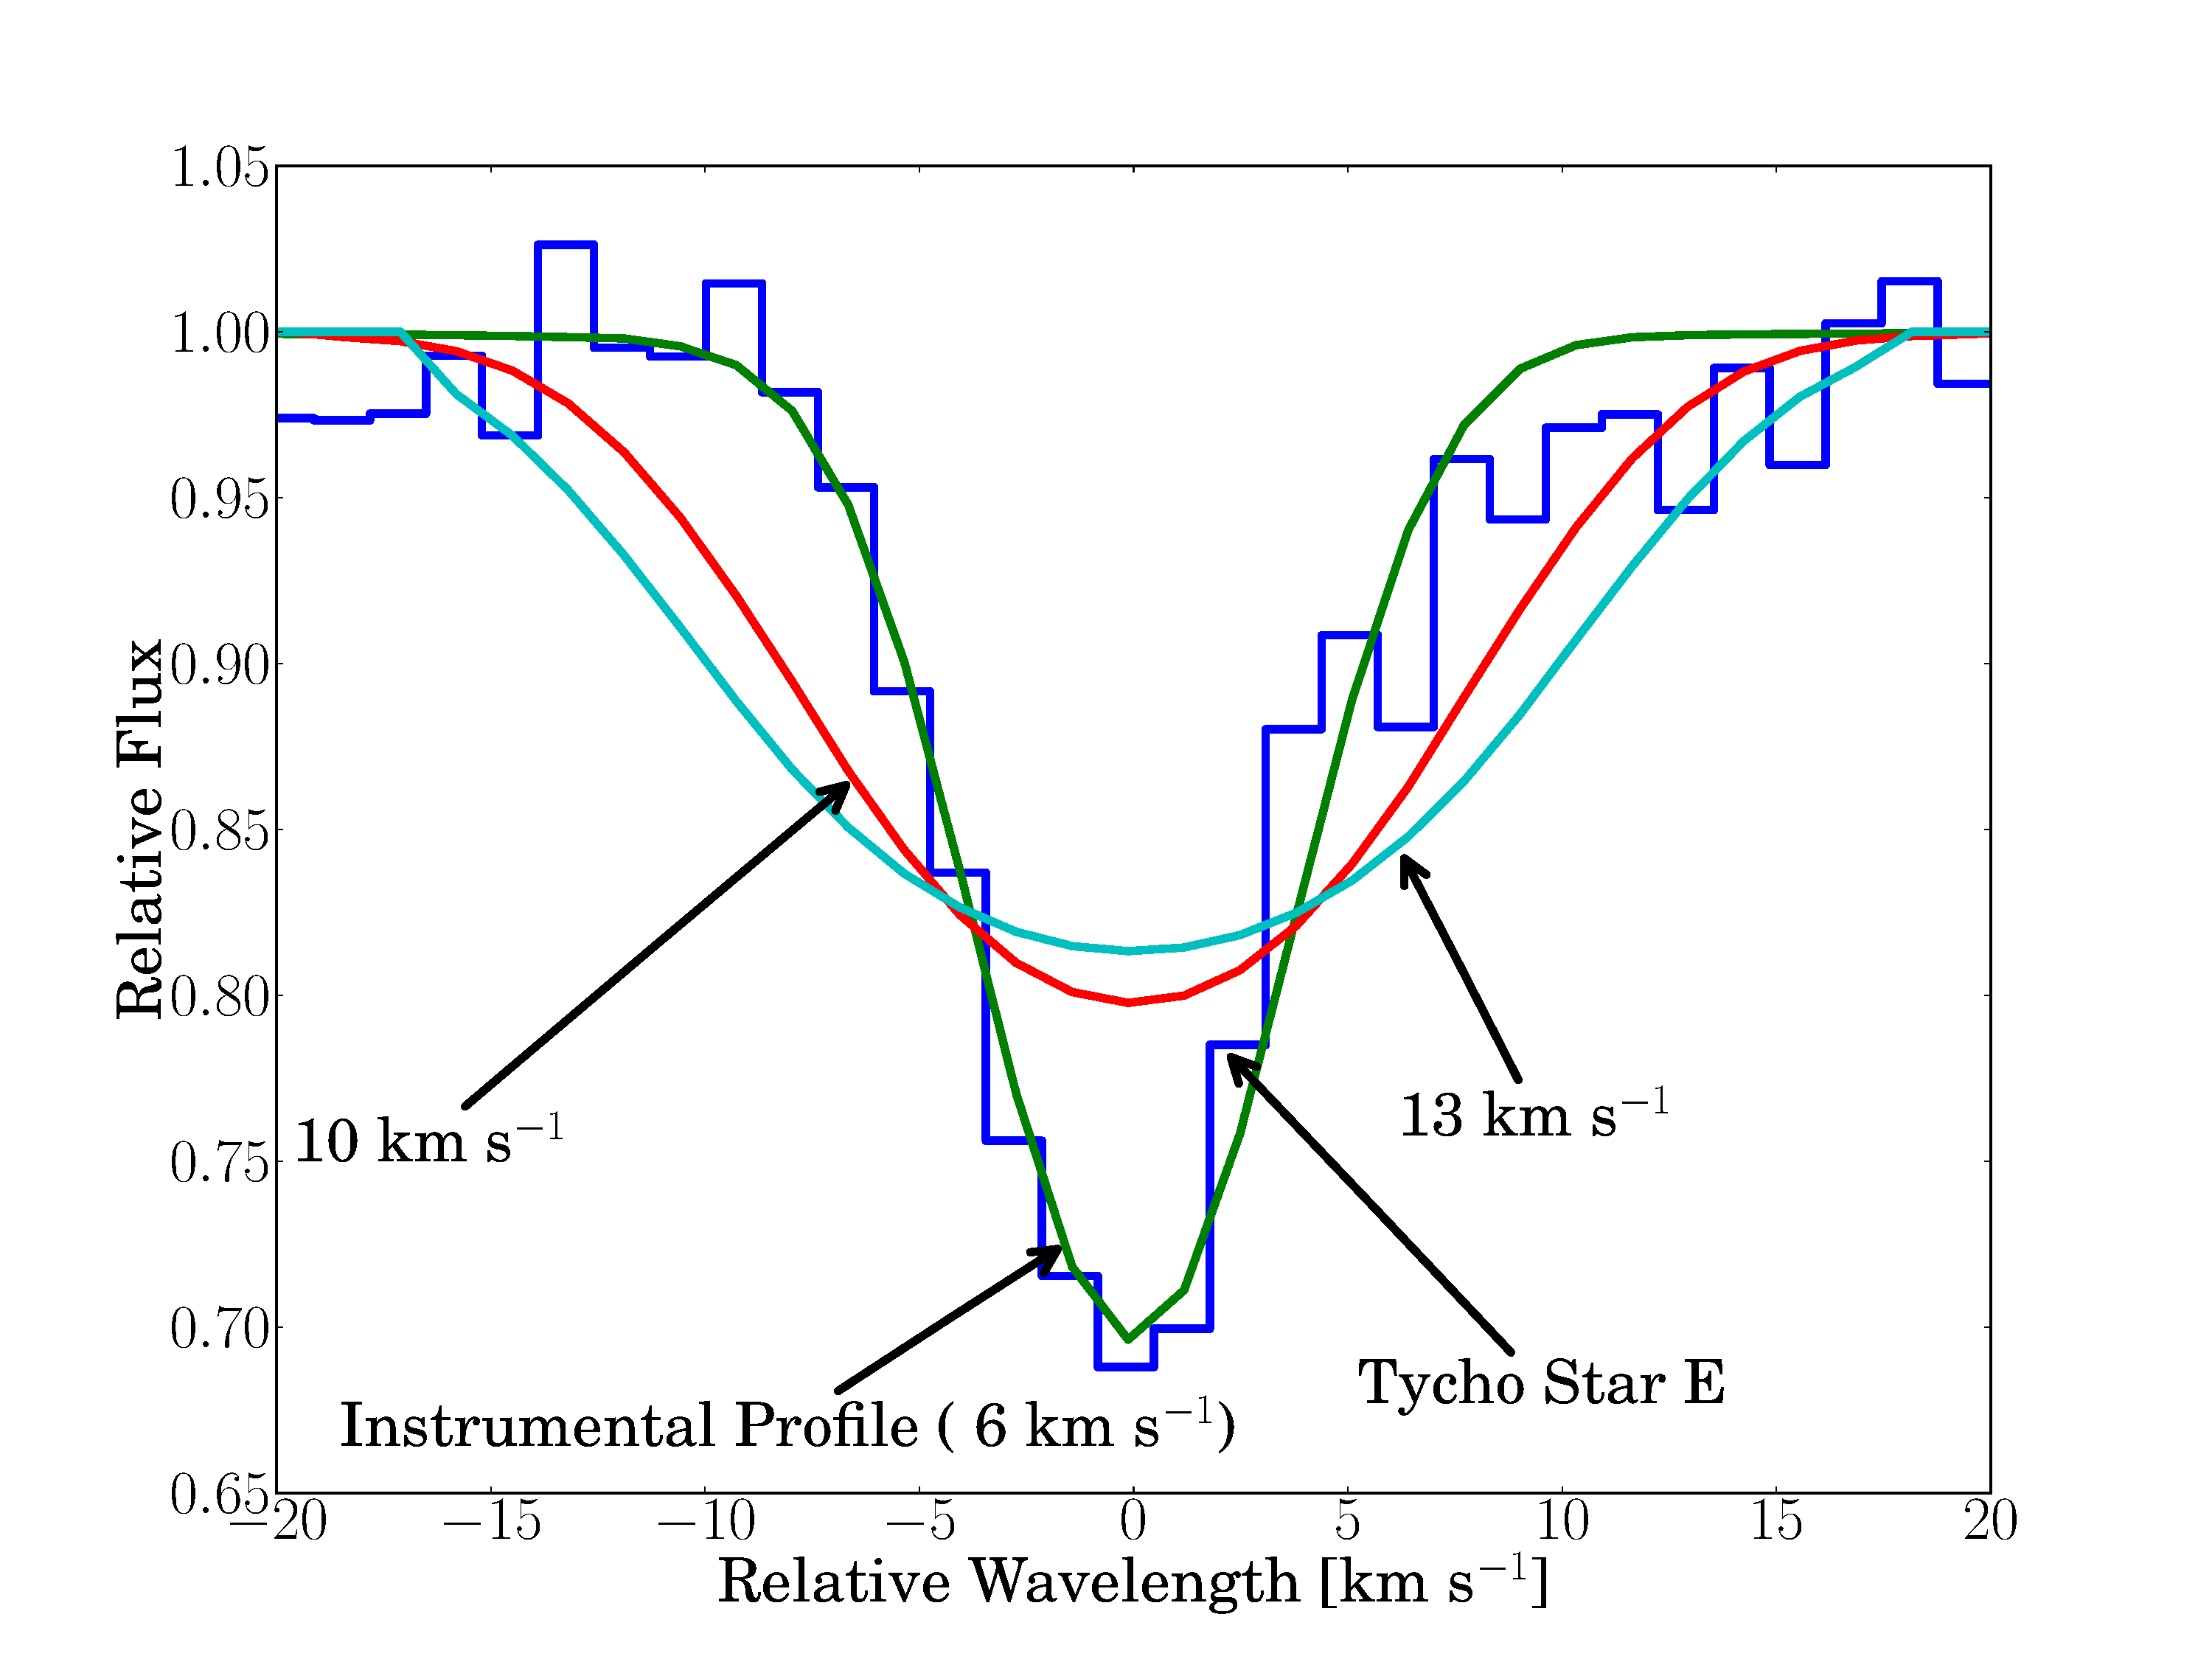
\includegraphics[width=0.45\textwidth, trim=130 30 60 0]{chapter3/plots/stare_rotation.pdf} &
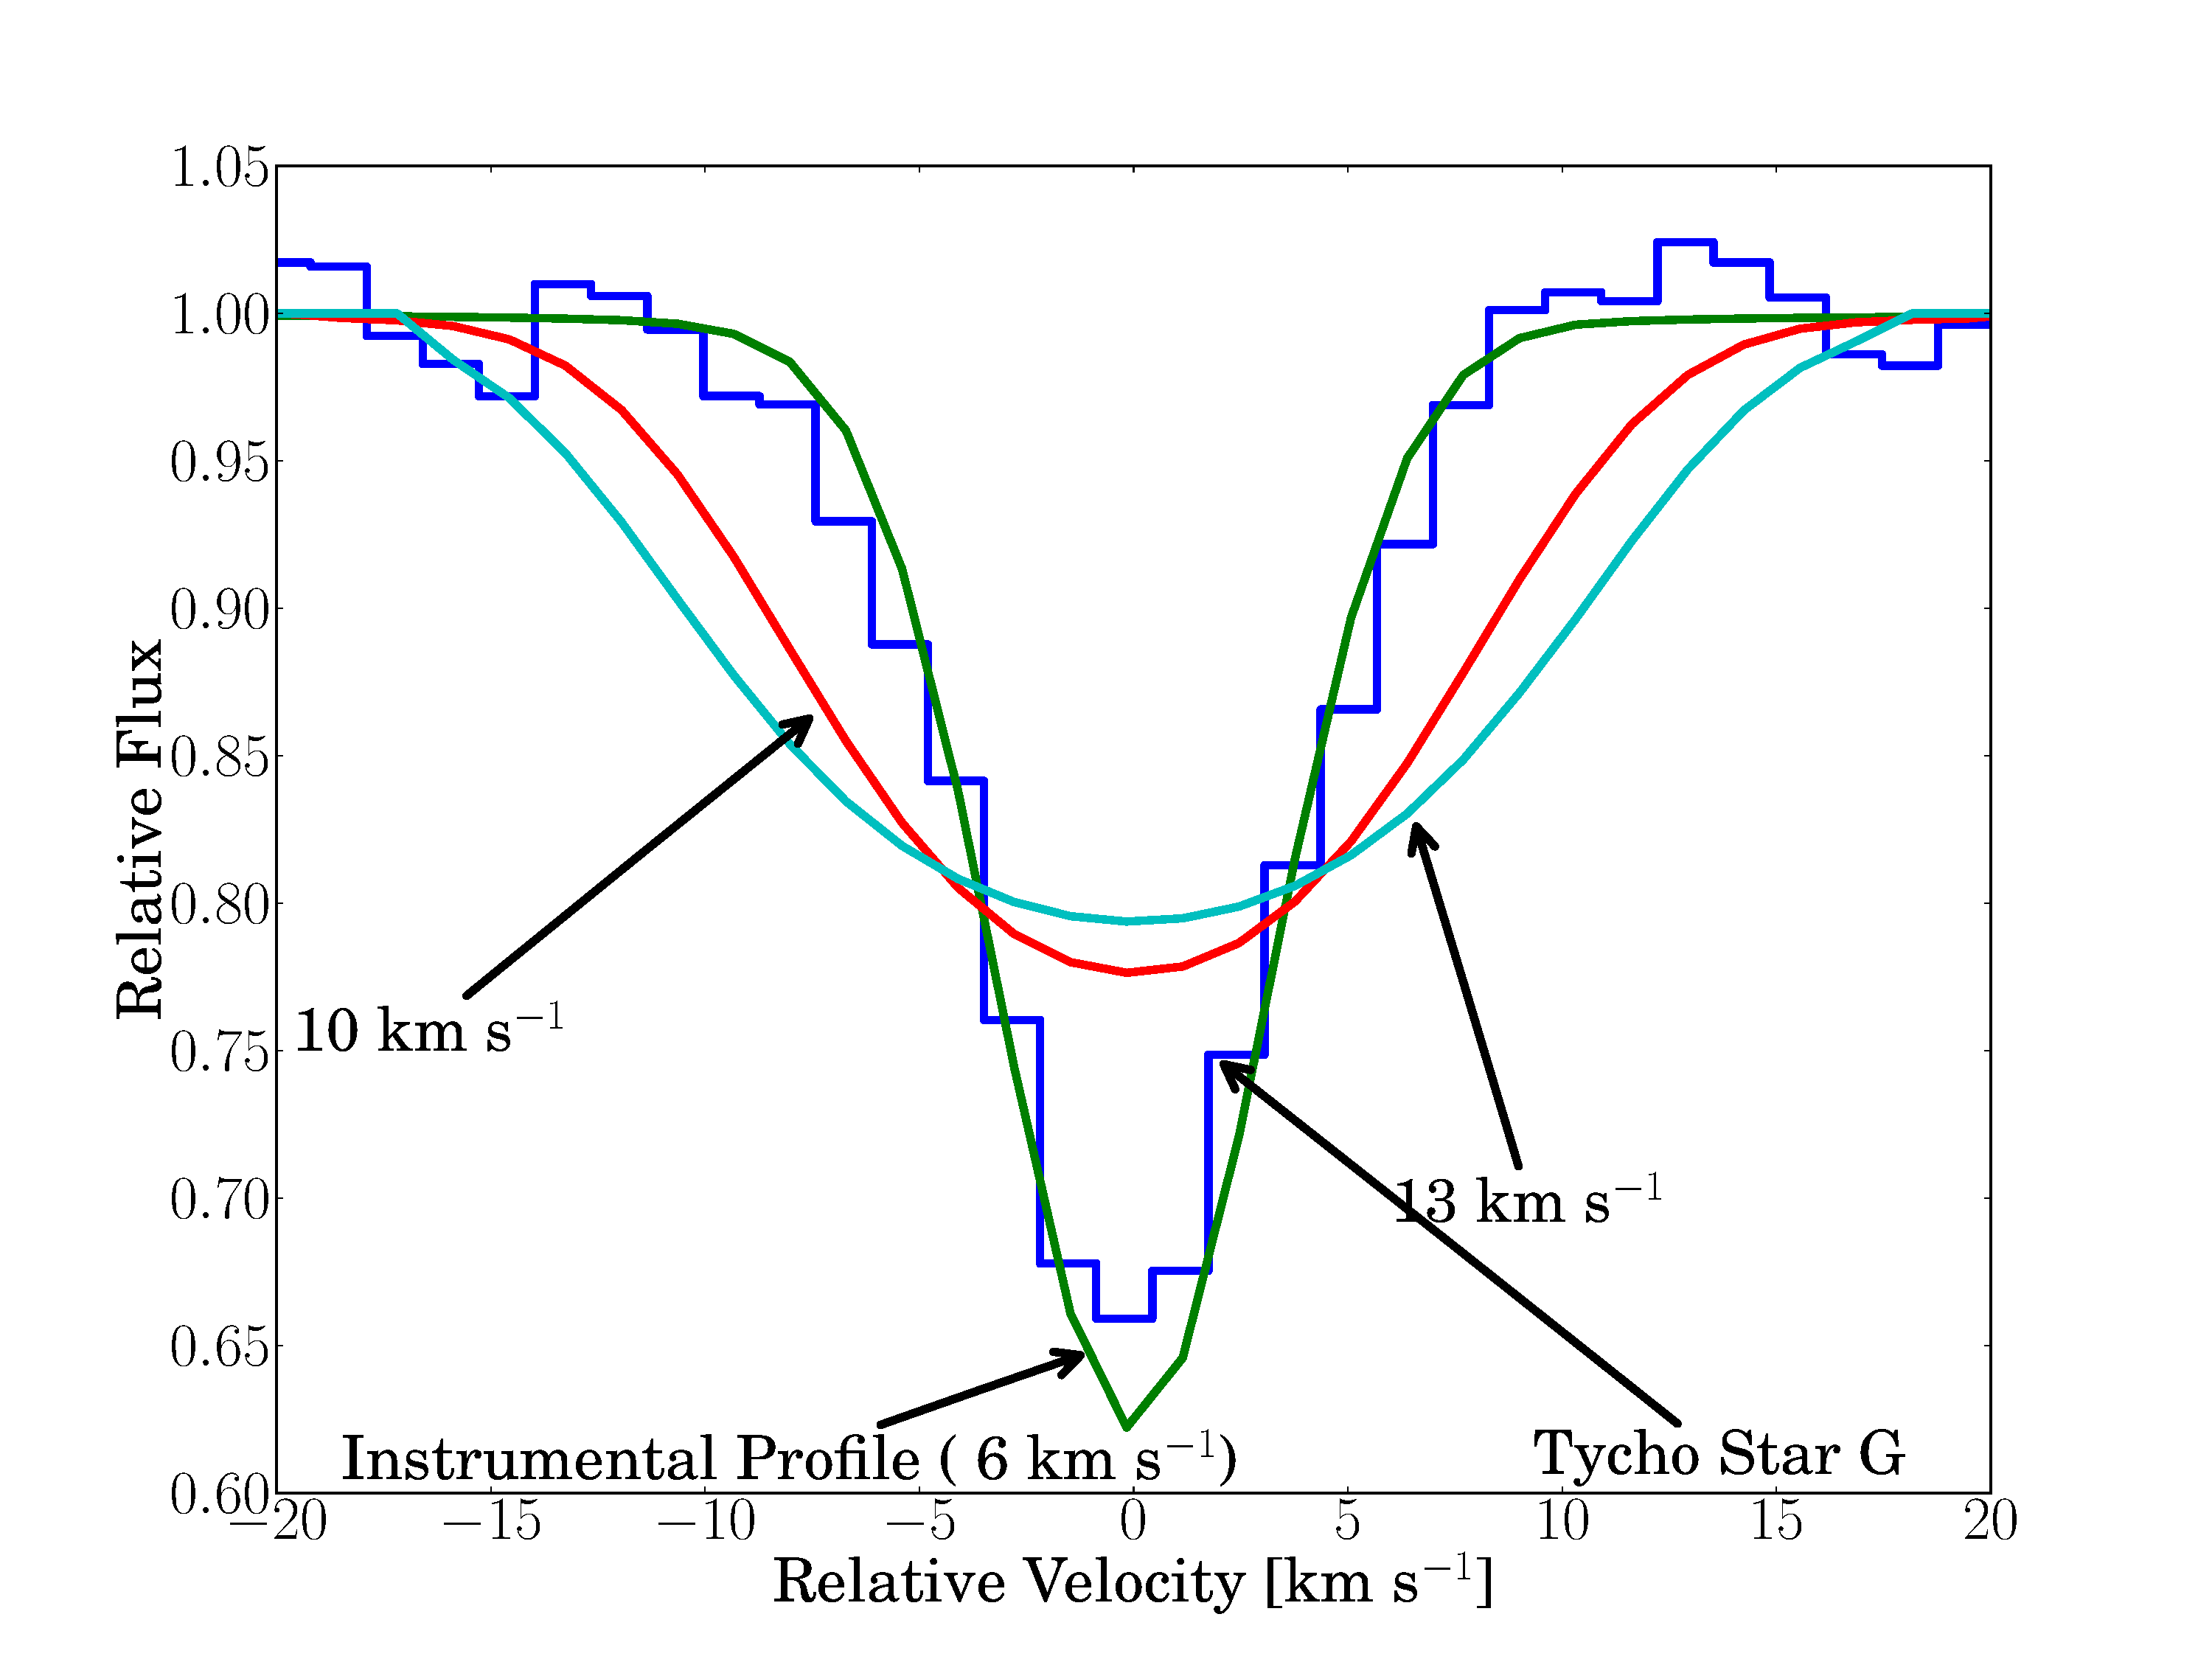
\includegraphics[width=0.45\textwidth, trim=130 30 60 0]{chapter3/plots/starg_rotation.pdf} \\
\end{tabular}
\caption{ The figures show the combination of Fe-line profiles after normalization to the same equivalent width and compare them to synthetic line profiles created by MOOG. We convolved the synthetic lines first with a rotational kernel with three different values for rotation and then with the instrumental profile. All stars show rotation less than 6 \kms\ which is equal to the instrumental profile at this resolution. }
\label{fig:rotvel}
\end{figure*}

\paragraph{\starb:}
We fit the rotational velocity for \starb\ with the program \textit{sfit}\ \citep[][described in section \ref{sec:stellar-parameters}]{2001A&A...376..497J}.  This resulted in $v_{\rm rot}=171^{+16}_{-33}$\,\kms. \starb's rotation is very high compared to the other candidate stars, however, for stars  of comparable stellar parameters, a high rotation is not unusual.


In summary, none of the stars show unusually high rotation.

%In addition, we measured the rotation of \starb\  with the broadening of  the oxygen triplet at 7777.1 \AA. 
%The triplet provides a unique structure that makes rotational measurements relatively straight forward. We
%synthesized a spectrum with MOOG \citemoog\ using LTE model atmospheres from the \citet{2003IAUS..210P.A20C} grid. We chose a $T_{\textnormal{eff}}=10000$\,K,  $\log{g}=3.7$ and $\textrm{[Fe/H]}=-1.0$. We then broadened it with the instrumental profile and three different rotational velocity kernels (50, 170 and 250\,\kms) shown in Figure \ref{fig:starb_rotcompare}. A velocity $v_{\textnormal{rot}} = 170$\kms\  is the best fitting rotational velocity.In addition, we measured a radial velocity while fitting \starb\ with \textit{sfit} \citesfit. 




\subsection{Stellar parameters}
\label{sec:stellar-parameters}
The stellar parameters are presented in Table \ref{table:stel_param} and were determined using a traditional spectroscopic approach. These measurements exclude \starb, which measurements will be described in a separate paragraph at the end of this section. 

Equivalent widths (EWs) for a set of Fe lines were measured using routines in IRAF (compiled from \citet[][henceforth Reddy03]{2003MNRAS.340..304R} and \citet[][henceforth RC02]{2002AJ....123.3277R} see Table \ref{table:llist}). We used the local thermodynamic equilibrium (LTE) stellar line analysis program MOOG \citemoog\ and LTE model atmospheres from the \citet{2003IAUS..210P.A20C} grid to derive an abundance for a given line. The effective temperature, \teff, was adjusted until the abundances from \ion{Fe}{1} lines displayed no trend with the lower excitation potential. The surface gravity, \logg, was adjusted until the abundances from \ion{Fe}{1} and \ion{Fe}{2} lines were in agreement. The microturbulent velocity, $\xi _{t}$ , was adjusted until there was no trend between the abundances from \ion{Fe}{1} lines and EW. This process was iterated until self consistent stellar parameters were obtained. Ideally, the trends between abundance and EW as well as between abundance and lower excitation potential should be exactly zero (david: how far was it in our tests - rough number.....)???. Furthermore, the abundances $\log{\epsilon}$(\ion{Fe}{1}) and $\log{\epsilon}$(\ion{Fe}{2})  should be exactly the same. In our analysis, we explored stellar parameters at discrete values. For \teff, we considered values at every 25 K (e.g., 4000, 4025 K, etc.), for \logg , we considered values at every 0.05 dex (e.g., 1.00, 1.05 dex, etc.), and for $\xi _{t}$ , we considered values at every 0.05 \kms (e.g., 1.70, 1.75 \kms, etc.). We assumed that excitation equilibrium was satisfied when the slope between $\log{\epsilon}$(\ion{Fe}{1}) and lower excitation potential $(\chi)$ was $\leq0.004$. We assumed that ionization equilibrium was achieved when $\vert\log{\epsilon} ($\ion{Fe}{1}$) - \log{\epsilon} ($\ion{Fe}{2}$)\vert$ dex. The microturbulent velocity was set when the slope between $\log{\epsilon}$(\ion{Fe}{1}) and reduced equivalent width ($\log{\rm{W}}/\lambda$) was $\leq0.004$. We estimate that the internal errors are typically $T_{\rm{eff}}\pm100$\,K, $\log{g}\pm0.3$\,dex, and $\xi _{t}\pm0.3$\,\kms (perhaps smaller for \stara\ and larger for \starc\ due to S/N considerations). 
For further details regarding the derivation of stellar parameters, see \citet{2008ApJ...673..854Y}.

The final iron measurements are the average of \ion{Fe}{1} and \ion{Fe}{2} assuming the solar abundances of \citet{2009ARA&A..47..481A} 
In addition, we measured abundance for the Elements Ni and Li via EW analysis. GH09 claimed that due to contamination of the star with the ejecta the levels of these elements could be enhanced. We could not see any unusual abundance pattern for any of the sample stars (see Figure \ref{fig:kobayashi06}; \starb's abundances are not presented on the plot as they were measured in a different fashion).  The line list (see Table \ref{table:llist}) for the Fe lines includes $\log{gf}$-values, sources and measured EWs.


%\begin{deluxetable}{cccccccc}
%
%\tablecaption{Stellar Parameters  \label{table:stel_param}}
%
%
%\tablehead{\colhead{Name} & \colhead{Teff} & \colhead{logg} & \colhead{[Fe/H]} & \colhead{$\Delta$[Fe/H]} & \colhead{[Ni/H]} & \colhead{$\Delta$[Ni/H]} & \colhead{[Li/H]} \\ 
%\colhead{} & \colhead{(K)} & \colhead{(dex)} & \colhead{(dex)} & \colhead{(dex)} & \colhead{(dex)} & \colhead{(dex)} & \colhead{(dex)} } 
%
%\startdata
%\stara & 4975 & 2.9 & 0.02 & 0.16 & 0.05 & 0.025 & 0.09 \\
%\starc & 4950 & 2.9 & -0.57 & 0.23 & -0.14 & -0.17 & 0.11 \\
%\stare & 5825 & 3.4 & -0.16 & 0.21 & 0.2 & 0.0 & 0.131\\
%\starg & 6025 & 4 & -0.15 & 0.18 & 0.14 & 0.08 & 0.11 \\
%\enddata
%
%\end{deluxetable}


\begin{figure}[h] %  figure placement: here, top, bottom, or page
   \centering
   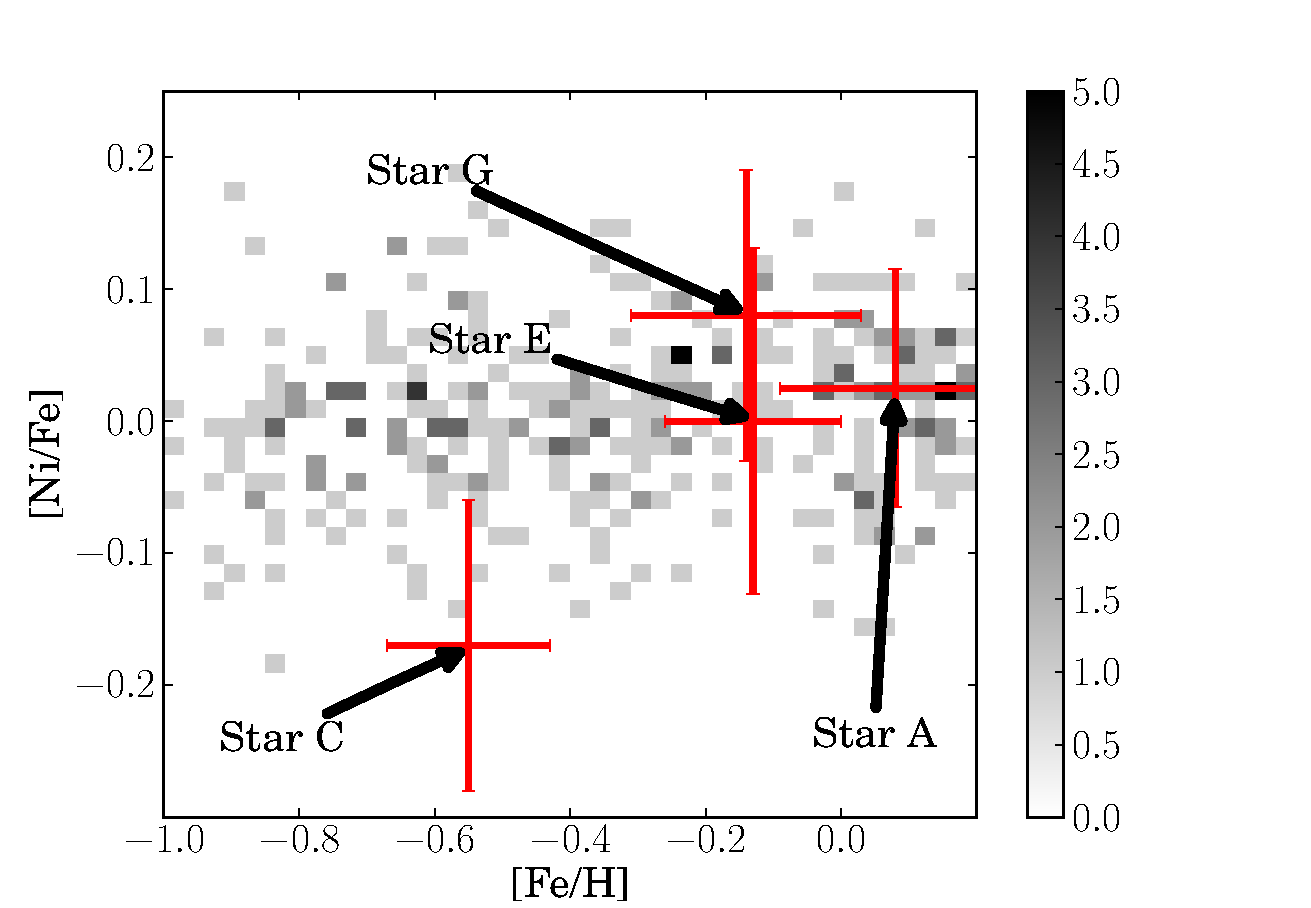
\includegraphics[width=1\textwidth]{chapter3/plots/abund_chiaki.pdf} 
   \caption{The background colour indicates the distribution is taken from \citet{2006ApJ...653.1145K}. All of the measured candidates are consistent within the errors with stars of the same metallicity.}
   \label{fig:kobayashi06}
\end{figure}

In summary, the inferred metallicities for all candidates show that the candidates are of roughly solar metallicities with the exception of the metal-poor \starc. The range of metallicities spanned by the program stars is compatible with membership of the thin disk (REFERENCE). Based on metallicity alone, we do not regard any of the program stars to be unusually metal-poor or metal-rich.  Additionally, we find the [Ni/Fe] abundance to be consistent with stars of similar metallicity (see Figure \ref{fig:kobayashi06}). The stellar paramaters and elemental abundances are listed in Table \ref{table:stel_param}.

\paragraph{\starb:} As \starb\ is the most unusual star in this set and very close to the 
remnants center we took two approaches to determine its parameters.  

We used the program \textit{sfit} \citesfit\ to match the HIRES-spectrum to a grid of model spectra. To determine the stellar parameters for \starb\ we have used a model grid with $\textnormal{[Fe/H]} = -1.0$, $8000 < T_{\textnormal{eff}} < 16000$, $7 < \log{g} < 2$. We used N(He) = 0.1 as this is empirically the most common He ratio in the universe. 
This analysis resulted in $T_{\rm eff} = 10000^{+ 400}_{-200}\,\rm{K}$, $\log{g} = 3.67$ with slope  $\partial \log{g}/\partial T_{\rm eff} = 0.27/500 \,\rm{K}^{-1}= 5.4 \times 10^{-4}\, \rm{K}^{-1}$, rotational velocity $v\sin{i} = 171$\,\kms\ with slope $\partial v\sin{i}/\partial T_{\rm eff} = -41/500\,\rm{km\,s^{-1}\,K^{-1}} =  -0.082\,\rm{km\,s^{-1}\,K^{-1}}$. From qualitative analysis this object seems metal poor (e.g. in comparison to stars of similar stellar parameters but solar metallicity), but its high rotation and general state make it hard to determine this parameter precisely. For the present, we assume [Fe/H] = -1.0 unless otherwise noted.

In addition, using the high-resolution spectrum, we measured the equivalent widths of several lines predicted to be strong in the VALD database \citep{2000BaltA...9..590K}. The abundances were deduced from the equivalent widths using a model atmosphere having $T_{\rm eff} = 10000$\,K, $\log{g}=3.67$ and [Fe/H] = -1.0 (see Table \ref{table:starb-abund}).

One caveat regarding these abundances is the use of equivalent widths from 
single lines with large rotational broadening, since the effect of blending 
with nearby weak lines cannot be taken into account. A second is that these 
abundances invariably rely on the strongest lines, which are precisely those 
most susceptible to departures from local thermodynamic equilibrium. 
Nevertheless, they do confirm the earlier impression that the star is 
metal-poor, and justify the adoption of [Fe/H]=$-1.0 \pm 0.4$


%\begin{deluxetable}{ccccccc}
%\tablecaption{\starb\ abundances}
%
%\tablehead{\colhead{Ion}&\colhead{$\lambda$}& \colhead{$W_{\lambda}$}& \colhead{$\epsilon$} & $[X/H]$ & \colhead{$\frac{\partial \epsilon}{\partial \log{g}}$}  &\colhead{$\frac{\partial \epsilon}{\partial T_{\rm eff}}$}\\
%			\colhead{}& \colhead{\AA} & \colhead{\AA} & \colhead{dex} & \colhead{dex}& \colhead{}&\colhead{K$^-1$}} 
%
%\startdata
%\ion{Mg}{2} & 4481.13+4481.33 & $220\pm15$ & $6.18\pm.08$ & -1.40&0.08&$8\times10^{-5}$ \\ 
%\ion{Si}{2} & 6347.1 & $140\pm5$ & $6.96\pm.18$ & -0.59&-0.02&$1\times10^{-4}$\\
%\ion{O}{1} & 7771.9+7774.2+7775.4 & $460\pm30$ & $8.43\pm.10$ & -0.58 &0.24&$-4\times10^{-5}$\\
%\enddata
%
%\label{table:starb-abund}
%
%\end{deluxetable}

As a second approach to determine the stellar parameters of \starb\ we used the low resolution spectra observed with LRIS.  The observation range of LRIS was chosen to be centered around the Balmer jump as this feature is sensitive to the surface gravity \citep{2007PASP..119..605B}. We fitted the spectra to a grid of model spectra \citep[]{2005A&A...442.1127M} by using our internal spectrum fitting tool. The final grid we used covered $\log{g}$ from 3.5 to 4.5 in steps of 0.5 and \teff\ from 9000 to 12000\,K in steps of 500\,K. In addition we expanded the grid by reddening the spectra with the \textit{pysynphot}-package\footnote{pysynphot is a product of the Space Telescope Science Institute, which is operated by AURA for NASA.}. We also added diffuse interstellar bands  \citep{1937PASP...49..224B, 1966ZA.....64..512H, 1967IAUS...31...85H, 1975ApJ...196..129H, 1995ARA&A..33...19H, 1994dib..nasa...31H, 1994A&AS..106...39J, 1958ApJ...128...57W} to the synthetic spectra , which were scaled with reddening . The included E(B-V) ranged from 0.5 to 1.3 in steps of 0.2. We assumed a rotation of 171\,\kms\ in the grid  (see section \ref{sec:rotation}).

We used the sum-squared difference of the grid to the spectrum of \starb\ as the figure of merit in our fitting procedure. To find the best fit for \starb\ we used the simplex algorithm provided by \textit{MINUIT} \citep{James:1975dr} and linearly interpolated between the grid points using the \textit{QHULL} algorithm described in \citet{Barber96thequickhull}. The grid fits the observations poorly in the wavelength region between 3800 -- 4280 \AA\ in (see Figure \ref{fig:starb_spec_comp}). Thus we excluded this region in our fit and find \teff=10799\,K, \logg=4.1, \feh=-1.5 and E(B-V)=0.87. We have also fitted \starb\ including the wavelength region between 3800 -- 4280 \AA\ which resulted in \teff=10579\,K, \logg=4.0, \feh=-1.5 and E(B-V)=0.85. We believe that the differences are indicative of the systematic errors in the fit. For future reference, however, we will us the best fit where we excluded the problematic wavelength region. When exploring the parameter space we also discovered that [Fe/H] is not very well constrained, although they match in this particular instance.



\begin{figure*}[h!]

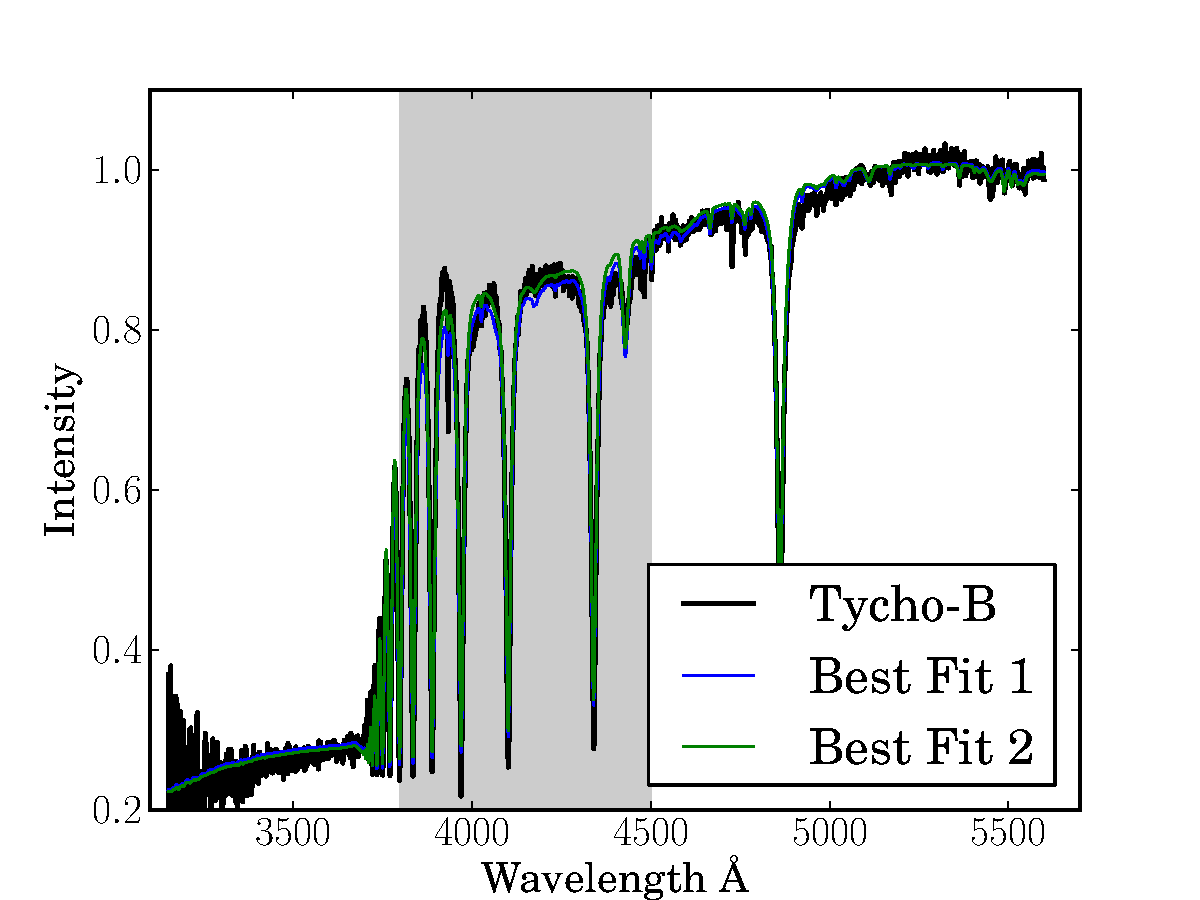
\includegraphics[width=1.\textwidth]{chapter3/plots/starb_spec_comp.pdf} 

\caption{The plot shows the normalized spectrum of \starb\ with the fit which excluded the spectral region between 3800 -- 4500 \AA (Best Fit 1) and the fit with the problematic region (Best Fit 2). The region is marked with a gray shade.  }
\label{fig:starb_spec_comp}
\end{figure*}

\subsection{Distance}
\label{sec:distance}
To measure the distance to the candidate stars we used colours and absolute magnitude from isochrones by  \citet{2004ApJ...612..168P}. We used the MIGRAD algorithm  \citep{James:1975dr} to find close matches of the measured values to \teff-\logg\ isochrones by varying the age of the isochrone. The isochrones were explored in the age dimension. In addition we calculate E(B-V) using the isochrone's colour and we extract a mass from the isochrone. The results can be seen in Table \ref{table:iso_dist}. Errors included in Table \ref{table:iso_dist} are rough indicators, for proper analysis please see the error contours in Figure \ref{fig:mc_isochrone}.

To estimate the errors in all distance, reddening and mass we employed the Monte-Carlo method with 10,000 samples of \teff, \logg, \feh, B- and V-magnitude (see Figure \ref{fig:mc_isochrone}). 

The data shows that all stars are compatible with the distance of the remnant. This is not unexpected as the uncertainties of the measurements in stellar parameters are relatively large.




\begin{figure}[htbp] %  figure placement: here, top, bottom, or page
   \includegraphics[width=0.5\textwidth]{chapter3/plots/tycho-a-panel.pdf} 
   \includegraphics[width=0.5\textwidth]{chapter3/plots/tycho-b-panel.pdf} 
   \includegraphics[width=0.5\textwidth]{chapter3/plots/tycho-c-panel.pdf} 
   \includegraphics[width=0.5\textwidth]{chapter3/plots/tycho-e-panel.pdf} 
   \includegraphics[width=0.5\textwidth]{chapter3/plots/tycho-g-panel.pdf} 
   \caption{The figures show error contours for distance, extinction and mass of the candidates. The lower right shows the optimal isochrone \citep{2004ApJ...612..168P}  for the measured values of \teff\ and \logg. }
   \label{fig:mc_isochrone}
\end{figure}



%\begin{deluxetable}{ccccccc}
%\tablecaption{Iso distance}
%
%\tablehead{\colhead{Name}&\colhead{Mass}& \colhead{$\Delta$Mass} & \colhead{Age} & \colhead{$\Delta$Age} & \colhead{Distance}& \colhead{$\Delta$Distance}\\
%	            \colhead{}& \colhead{M/M$_\odot$} & \colhead{M/M$_\odot$} & \colhead{Gyr} & \colhead{Gyr} & \colhead{kpc} & \colhead{kpc}} 
%
%\startdata
%\stara & 2.4 & 0.8 &0.7 & 2.3 & 1.4 & 0.8\\
%\starb & 1.8 & 0.4 &0.8 & 0.3 & 1.8 & 0.8\\
%\starc & 0.9 & 0.4 &10.0 & 3.4 & 5.5 & 3.5\\
%\stare & 1.7 & 0.4 &1.4 & 1.1 & 11.2 & 7.5\\
%\starg & 1.1 & 0.2 &5.7 & 2.1 & 3.7 & 1.5\\
%\enddata
%
%\label{table:iso_dist}
%
%\end{deluxetable}


\section{Conclusion}
\label{sec:conclusion_sn1572_hires}

In our sample of six stars we find no star that is obvious as a a donor star for SN1572. On the other hand none of the stars in the sample can be completely ruled out. 

\stara\ is a metal rich giant which taking all measurements into account is very likely a foreground star. The only redeeming feature as a donor star candidate is that it is located in the geometric center of the remnant. \stara's kinematic signature however make it very hard to reconcile with any donor star model.

\starb's high rotational velocity and unusual chemical abundance made it one of the most interesting candidates in the set. It is located in the geometric center of the remnant. Many scenarios for the donor star include high rotation which \starb\ shows, but also include a high spatial velocity post-explosion. \starb\ does not show this high spatial velocity. ????Philipp what do we think it i????

\starc\ is a metalpoor giant which is located considerably away from the geometric center of the remnant. \starc\ consists of two stars which are only resolved in HST images. It consists of a brighter bluer component and a dimmer redder component (difference of ~ one magnitude in all colors) (\rl). \starc\ does not have any features compared to the rest of the sample that make it likely as a donor star candidate.

\stard\ is roughly ten times dimmer than the close star \starc\ ($\approx 0.6$\arcsec). Our tools to measure stellar abundances are not effective for spectra with a S/N less than 10. We however compared the stars by over plotting them and determined that \stard\ is similar to \starc. 

\stare\ is the most distant star in this set (11.2\,kpc). It seems to be similar to  Tycho-G in temperature, however is a subgiant. It is located far away from the geometric center and has no unusual stellar parameters or kinematics.

\starg\, for our set, is the star furthest away from the geometric center. It is a solar metallicity subgiant and is distance compatible with the remnant. It has an unusually high proper motion, but has a radial velocity which is consistent with that of a background interloper. \starg\ does not show any unusual elemental abundance and no unusually large rotation. Reconciling the large distance to the geometric center in the plane of the sky makes it very hard to reconcile it with common donor star models.

In summary, we do not see any obvious donor star candidate in Tycho's remnant. We do acknowledge that \starb\ is an unusual star and certainly does have features that would fit well with a donor star model. On the other hand it's lack of high spatial velocity and the suggested distance seem to make it hard to reconcile it with common donor star scenarios. 
\starg's only redeeming feature is that it is an outlier in proper motion. We could not reproduce the reported enhanced abundance in Nickel or Lithium reported by \gh. When trying to reconcile \starg\ with a donor scenario our main concerns are the relatively large distance from the geometric center, lack of rotation and consistency with a background interloper model (see section \ref{sec:stellar-parameters}).

\section{Acknowledgments}
\label{sec:acknowledgments}
PYRAF, scipy numpy matplotlib ipython suite, kudritzki, peter wood (for fxcor),Jorge, Onken with HIRES stuff, Amanda with differential rotation


%\begin{deluxetable}{cccccccc}
%
%\tablecaption{Measured equivalent widths from the Keck HIRES spectra.\label{table:llist}}
%
%\tablehead{\colhead{$\lambda$} & \colhead{$\chi$} & \colhead{$\log{gf}$} & \colhead{Source} & \colhead{\stara} & \colhead{\starg} & \colhead{\starc} & \colhead{\stare} \\ 
%\colhead{(\AA)} & \colhead{(eV)} & \colhead{(dex)} & \colhead{} & \colhead{(dex)} & \colhead{(dex)} & \colhead{(dex)} & \colhead{(dex)} } 
%
%\startdata
%5082.35 & 3.658 & -0.59 & Reddy03 & 6.31 & 6.44 & \nodata & 6.2 \\
%5088.54 & 3.85 & -1.04 & Reddy03 & 6.19 & 6.33 & \nodata & \nodata \\
%5088.96 & 3.68 & -1.24 & Reddy03 & 6.21 & \nodata & \nodata & \nodata \\
%5094.42 & 3.83 & -1.07 & Reddy03 & 6.1 & \nodata & \nodata & \nodata \\
%5115.4 & 3.834 & -0.28 & Reddy03 & 6.22 & \nodata & \nodata & \nodata \\
%5682.20 & 4.10 & -0.47 & RC02 & 6.34 & \nodata & \nodata & \nodata \\
%5748.351 & 1.68 & -3.26 & RC02 & 6.33 & \nodata & 5.74 & \nodata \\
%5749.297 & 3.94 & -1.99 & RC02 & 6.38 & \nodata & \nodata & \nodata \\
%5847.01 & 1.676 & -3.41 & Reddy03 & 6.26 & \nodata & 5.55 & \nodata \\
%6007.31 & 1.68 & -3.34 & RC02 & 6.2 & \nodata & 5.45 & \nodata \\
%6053.685 & 4.23 & -1.07 & RC02 & 6.33 & \nodata & \nodata & \nodata \\
%6086.28 & 4.26 & -0.52 & RC02 & 6.25 & 6.22 & \nodata & \nodata \\
%6108.116 & 1.68 & -2.44 & RC02 & 6.26 & 6.11 & 5.33 & \nodata \\
%6111.08 & 4.088 & -0.81 & Reddy03 & 6.33 & \nodata & 5.38 & \nodata \\
%6130.14 & 4.266 & -0.94 & Reddy03 & 6.31 & \nodata & \nodata & \nodata \\
%6175.37 & 4.089 & -0.55 & Reddy03 & 6.25 & 6.35 & 5.7 & \nodata \\
%6176.82 & 4.09 & -0.26 & Reddy03 & 6.3 & 6.27 & 5.43 & 6.01 \\
%6177.25 & 1.83 & -3.51 & Reddy03 & 6.23 & \nodata & \nodata & \nodata \\
%6186.71 & 4.10 & -0.97 & RC02 & 6.33 & 6.23 & \nodata & \nodata \\
%6204.61 & 4.09 & -1.11 & Reddy03 & 6.32 & \nodata & \nodata & \nodata \\
%6322.17 & 4.15 & -1.17 & RC02 & 6.31 & \nodata & \nodata & \nodata \\
%6370.346 & 3.54 & -1.94 & RC02 & 6.37 & \nodata & \nodata & \nodata \\
%6378.26 & 4.154 & -0.83 & Reddy03 & 6.3 & \nodata & 5.81 & \nodata \\
%6482.80 & 1.93 & -2.63 & RC02 & 6.2 & \nodata & 5.38 & \nodata \\
%6598.60 & 4.23 & -0.98 & RC02 & 6.3 & \nodata & 5.74 & \nodata \\
%6635.12 & 4.42 & -0.83 & RC02 & 6.37 & \nodata & \nodata & \nodata \\
%\\
%6643.64 & 1.68 & -2.03 & Reddy03 & 6.48 & 6.02 & 5.34 & 5.97 \\
%6767.772 & 1.83 & -2.17 & RC02 & 6.35 & 6.19 & 5.67 & \nodata \\
%6772.32 & 3.658 & -0.97 & Reddy03 & 6.31 & \nodata & \nodata & \nodata \\
%6842.037 & 3.66 & -1.47 & RC02 & 6.4 & 6.36 & \nodata & \nodata \\
%7030.011 & 3.54 & -1.73 & RC02 & 6.42 & \nodata & \nodata & \nodata \\
%7122.197 & 3.54 & 0.048 & RC02 & 6.33 & \nodata & 5.34 & \nodata \\
%7261.918 & 1.95 & -2.7 & RC02 & \nodata & 6.26 & \nodata & \nodata \\
%7327.648 & 3.8 & -1.77 & RC02 & 6.38 & 6.44 & \nodata & \nodata \\
%7409.35 & 3.8 & -0.1 & RC02 & \nodata & \nodata & 5.24 & \nodata \\
%7414.502 & 1.99 & -2.57 & RC02 & \nodata & 6.2 & 5.57 & 6.03 \\
%7422.275 & 3.63 & -0.129 & RC02 & 6.47 & \nodata & 5.32 & 5.84 \\
%7574.048 & 3.83 & -0.58 & RC02 & 6.3 & 5.97 & 5.12 & \nodata \\
%7748.89 & 3.7 & -0.38 & Reddy03 & 6.42 & 6.17 & 5.41 & 6.27 \\
%7788.93 & 1.95 & -2.42 & RC02 & \nodata & \nodata & 5.87 & 6.33 \\
%7797.59 & 3.9 & -0.35 & Reddy03 & 6.41 & 6.16 & 5.59 & 6.2 \\
%7917.44 & 3.74 & -1.5 & RC02 & \nodata & 6.14 & \nodata & \nodata \\
%\enddata
%
%
%\end{deluxetable}
